\documentclass[xcolor=table, 10pt, aspectratio=43]{beamer}

%\usepackage{arev}
\usepackage{amsmath,amssymb,amscd}
\usepackage{dsfont}
\usepackage{mathrsfs}
\usepackage{yfonts}
\usepackage{bm}
\usepackage{graphicx}
\usepackage{tabularx}
\usepackage{animate}
%\usepackage{ifthen}

%\usepackage{xeCJK}
%\usepackage{fontspec}
%\newfontfamily\cjkfont{PingFang SC}
%\setCJKmainfont{PingFang SC}
\newcolumntype{x}{>{\centering\arraybackslash}X}
\renewcommand{\arraystretch}{1.5}

\usepackage{tikz}
	\usetikzlibrary{calc}
	\usetikzlibrary{arrows,shapes, positioning, matrix}
	\usetikzlibrary{decorations.markings}
	\tikzstyle arrowstyle=[scale=1]
	\tikzstyle directed=[postaction={decorate,decoration={markings,
 	   mark=at position .15 with {\arrow[arrowstyle]{stealth}}}}]
\tikzstyle string=[thick,postaction={decorate,decoration={markings,
    mark=at position .55 with {\arrow[arrowstyle]{stealth}}}}]
\tikzstyle dual_string=[dashed,postaction={decorate,decoration={markings,
    mark=at position .55 with {\arrow[arrowstyle]{stealth}}}}]

\tikzstyle dw=[thick,postaction={decorate,decoration={markings,
    mark=at position 1 with {\arrow[arrowstyle]{stealth}}}}]
\tikzstyle group=[mbg]

\usepackage{pgffor}
\newcommand{\mb}[1]{\mathbf{#1}}
\renewcommand{\cal}[1]{\mathcal{#1}}

\newcommand{\ag}[2]{#1_\mb{#2}}
\newcommand{\cohosub}[1]{\scalebox{0.72}{\textswab{#1}}}
\newcommand{\cohosubsub}[1]{\scalebox{0.6}{\textswab{#1}}}
\newcommand{\coho}[1]{\textswab{#1}}


\mode<presentation>
{
  %\usetheme{Warsaw}
  % or ...
  %\useoutertheme{rectangle}
  \setbeamertemplate{frametitle}[default][center]
  \defbeamertemplate{itemize item}{flat}{\begin{pgfpicture}{-1ex}{0ex}{1ex}{2ex}
      \pgfpathcircle{\pgfpoint{0pt}{.6ex}}{0.6ex}
      \pgfusepath{fill}
    \end{pgfpicture}%
  }
  \defbeamertemplate{itemize subitem}{flat}{\footnotesize\raise0.5pt\hbox{\textbullet}}
  \defbeamertemplate{itemize subsubitem}{flat}{\footnotesize\raise0.5pt\hbox{\textbullet}}

  %\useinnertheme{circles}
  \setbeamertemplate{items}[flat]
  \setbeamertemplate{sections/subsections in toc}[circle]
  \setbeamertemplate{blocks}[rounded]
  \setbeamertemplate{title page}[default][colsep=-4bp,rounded=true]
  \setbeamertemplate{part page}[default][colsep=-4bp,rounded=true]
  \setbeamercovered{transparent}
  %\usecolortheme{spruce}
  %\definecolor{THU}{RGB}{116,61,130}
  \definecolor{mbg}{RGB}{0,0,160}
  \setbeamercolor*{palette primary}{fg=white,bg=mbg}
  \setbeamercolor*{titlelike}{parent=palette primary}
  \setbeamercolor*{structure}{fg=mbg}
  \setbeamercolor{frametitle}{fg=white,bg=mbg}
  % or whatever (possibly just delete it)
  \setbeamercolor{block title}{bg=mbg,fg=white}
  \setbeamercolor{block body}{bg=mbg!15}


  \addtobeamertemplate{navigation symbols}{}{ \hspace{1em}%
    \usebeamerfont{footline}%
    \insertframenumber / \inserttotalframenumber }
}


%\usepackage[english]{babel}
% or whatever

%\usepackage[latin1]{inputenc}
% or whatever

%\usepackage{times}
%\usepackage[T1]{fontenc}
% Or whatever. Note that the encoding and the font should match. If T1
% does not look nice, try deleting the line with the fontenc.

\title[EQMC] % (optional, use only with long paper titles)
{EMUS-QMC: Elective Momentum Ultra-Size Quantum Monte Carlo Method}

\author[Y Qi] % (optional, use only with lots of authors)
{Yang~Qi}
% - Give the names in the same order as the appear in the paper.
% - Use the \inst{?} command only if the authors have different
%   affiliation.

\institute[Fudan] % (optional, but mostly needed)
{
Department of Physics, Fudan University.
}
% - Use the \inst command only if there are several affiliations.
% - Keep it simple, no one is interested in your street address.

%\date{2016 Annual Meeting of Fudan CFTPP} % (optional, should be abbreviation of conference name)
%{Fudan University, Oct 13 2015}
\date{USTC, Jan. 12$^{\text{th}}$, 2018}
% - Either use conference name or its abbreviation.
% - Not really informative to the audience, more for people (including
%   yourself) who are reading the slides online

\subject{Theoretical Physics}
% This is only inserted into the PDF information catalog. Can be left
% out.



% If you have a file called "university-logo-filename.xxx", where xxx
% is a graphic format that can be processed by latex or pdflatex,
% resp., then you can add a logo as follows:

\pgfdeclareimage[height=1cm]{university-logo}{../resources/fudan}
\logo{\pgfuseimage{university-logo}}



% Delete this, if you do not want the table of contents to pop up at
% the beginning of each subsection:
\AtBeginSection[]
{
  \begin{frame}<beamer>{Outline}
			\tableofcontents[currentsection,currentsubsection]
  \end{frame}
}
%\AtBeginSubsection[]
%{
 % \begin{frame}<beamer>{Outline}
  %  \tableofcontents[currentsection,currentsubsection]
  %\end{frame}
%}


\begin{document}

\begin{frame}
  \titlepage
  \begin{center}
    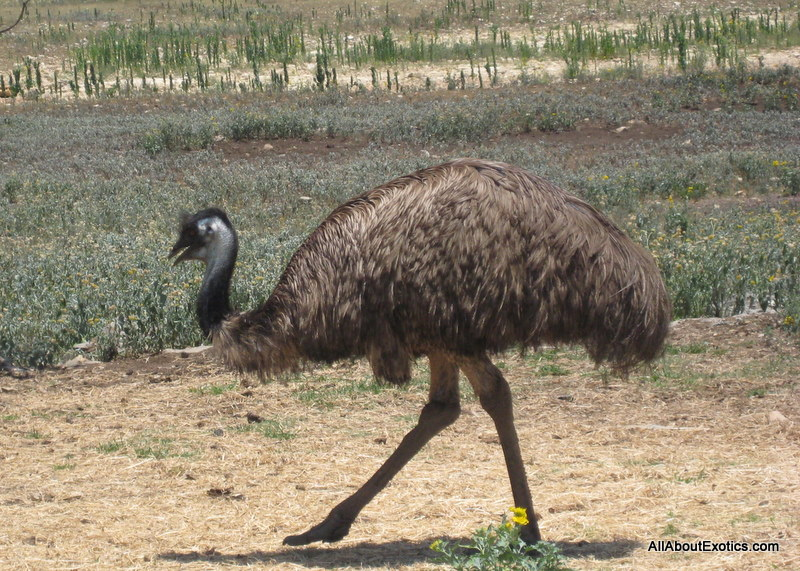
\includegraphics[height=3cm]{emu}
    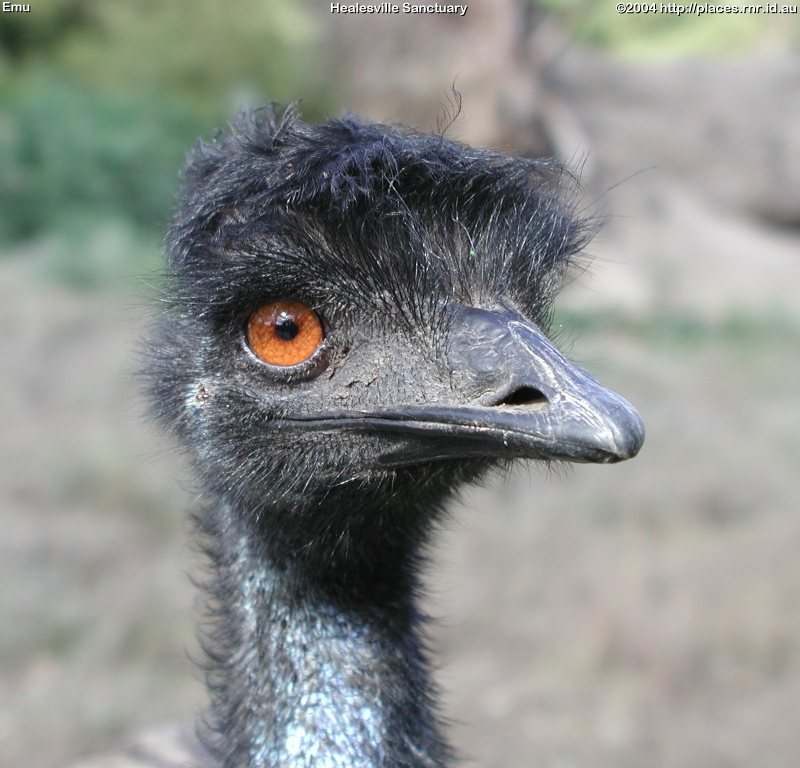
\includegraphics[height=3cm]{emu2}
  \end{center}
\end{frame}

\begin{frame}{Collaborators}
\begin{itemize}
\item Zi Hong Liu and Professor Zi Yang Meng, Institute of Physics.
\item Xiao Yan Xu, Hong Kong University of Science and Technology.
\item Kai Sun, University of Michigan, Ann Arbor.
\begin{center}
  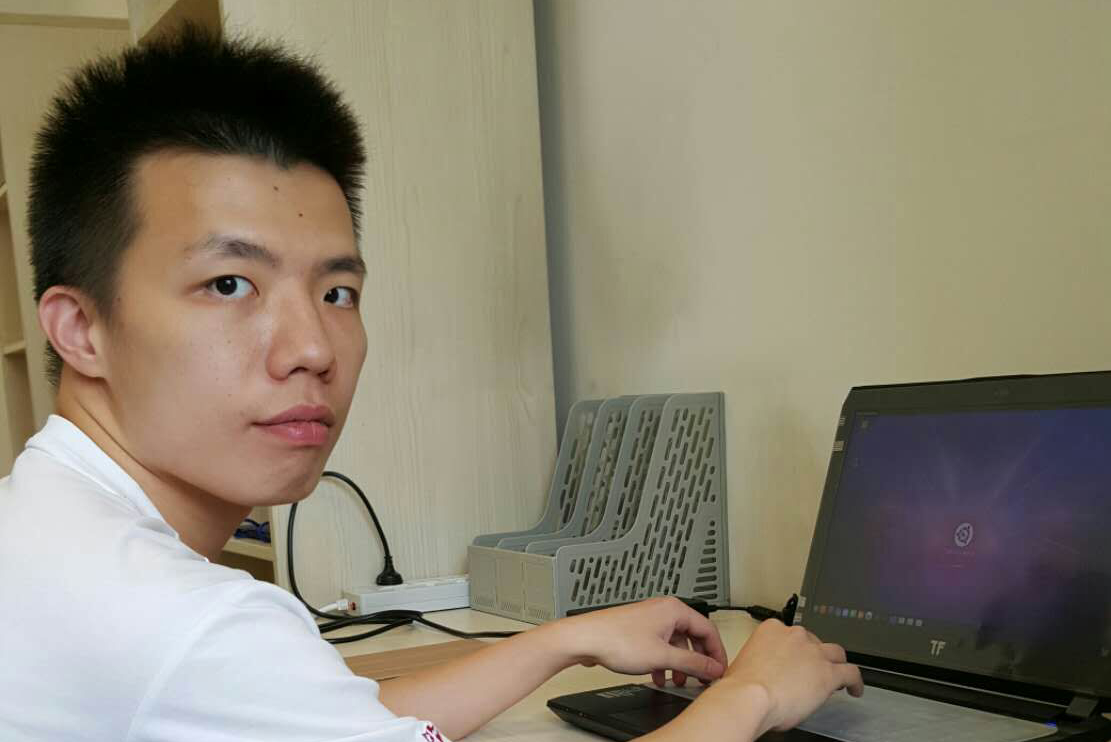
\includegraphics[height=2.5cm]{../people/zihongliu}
  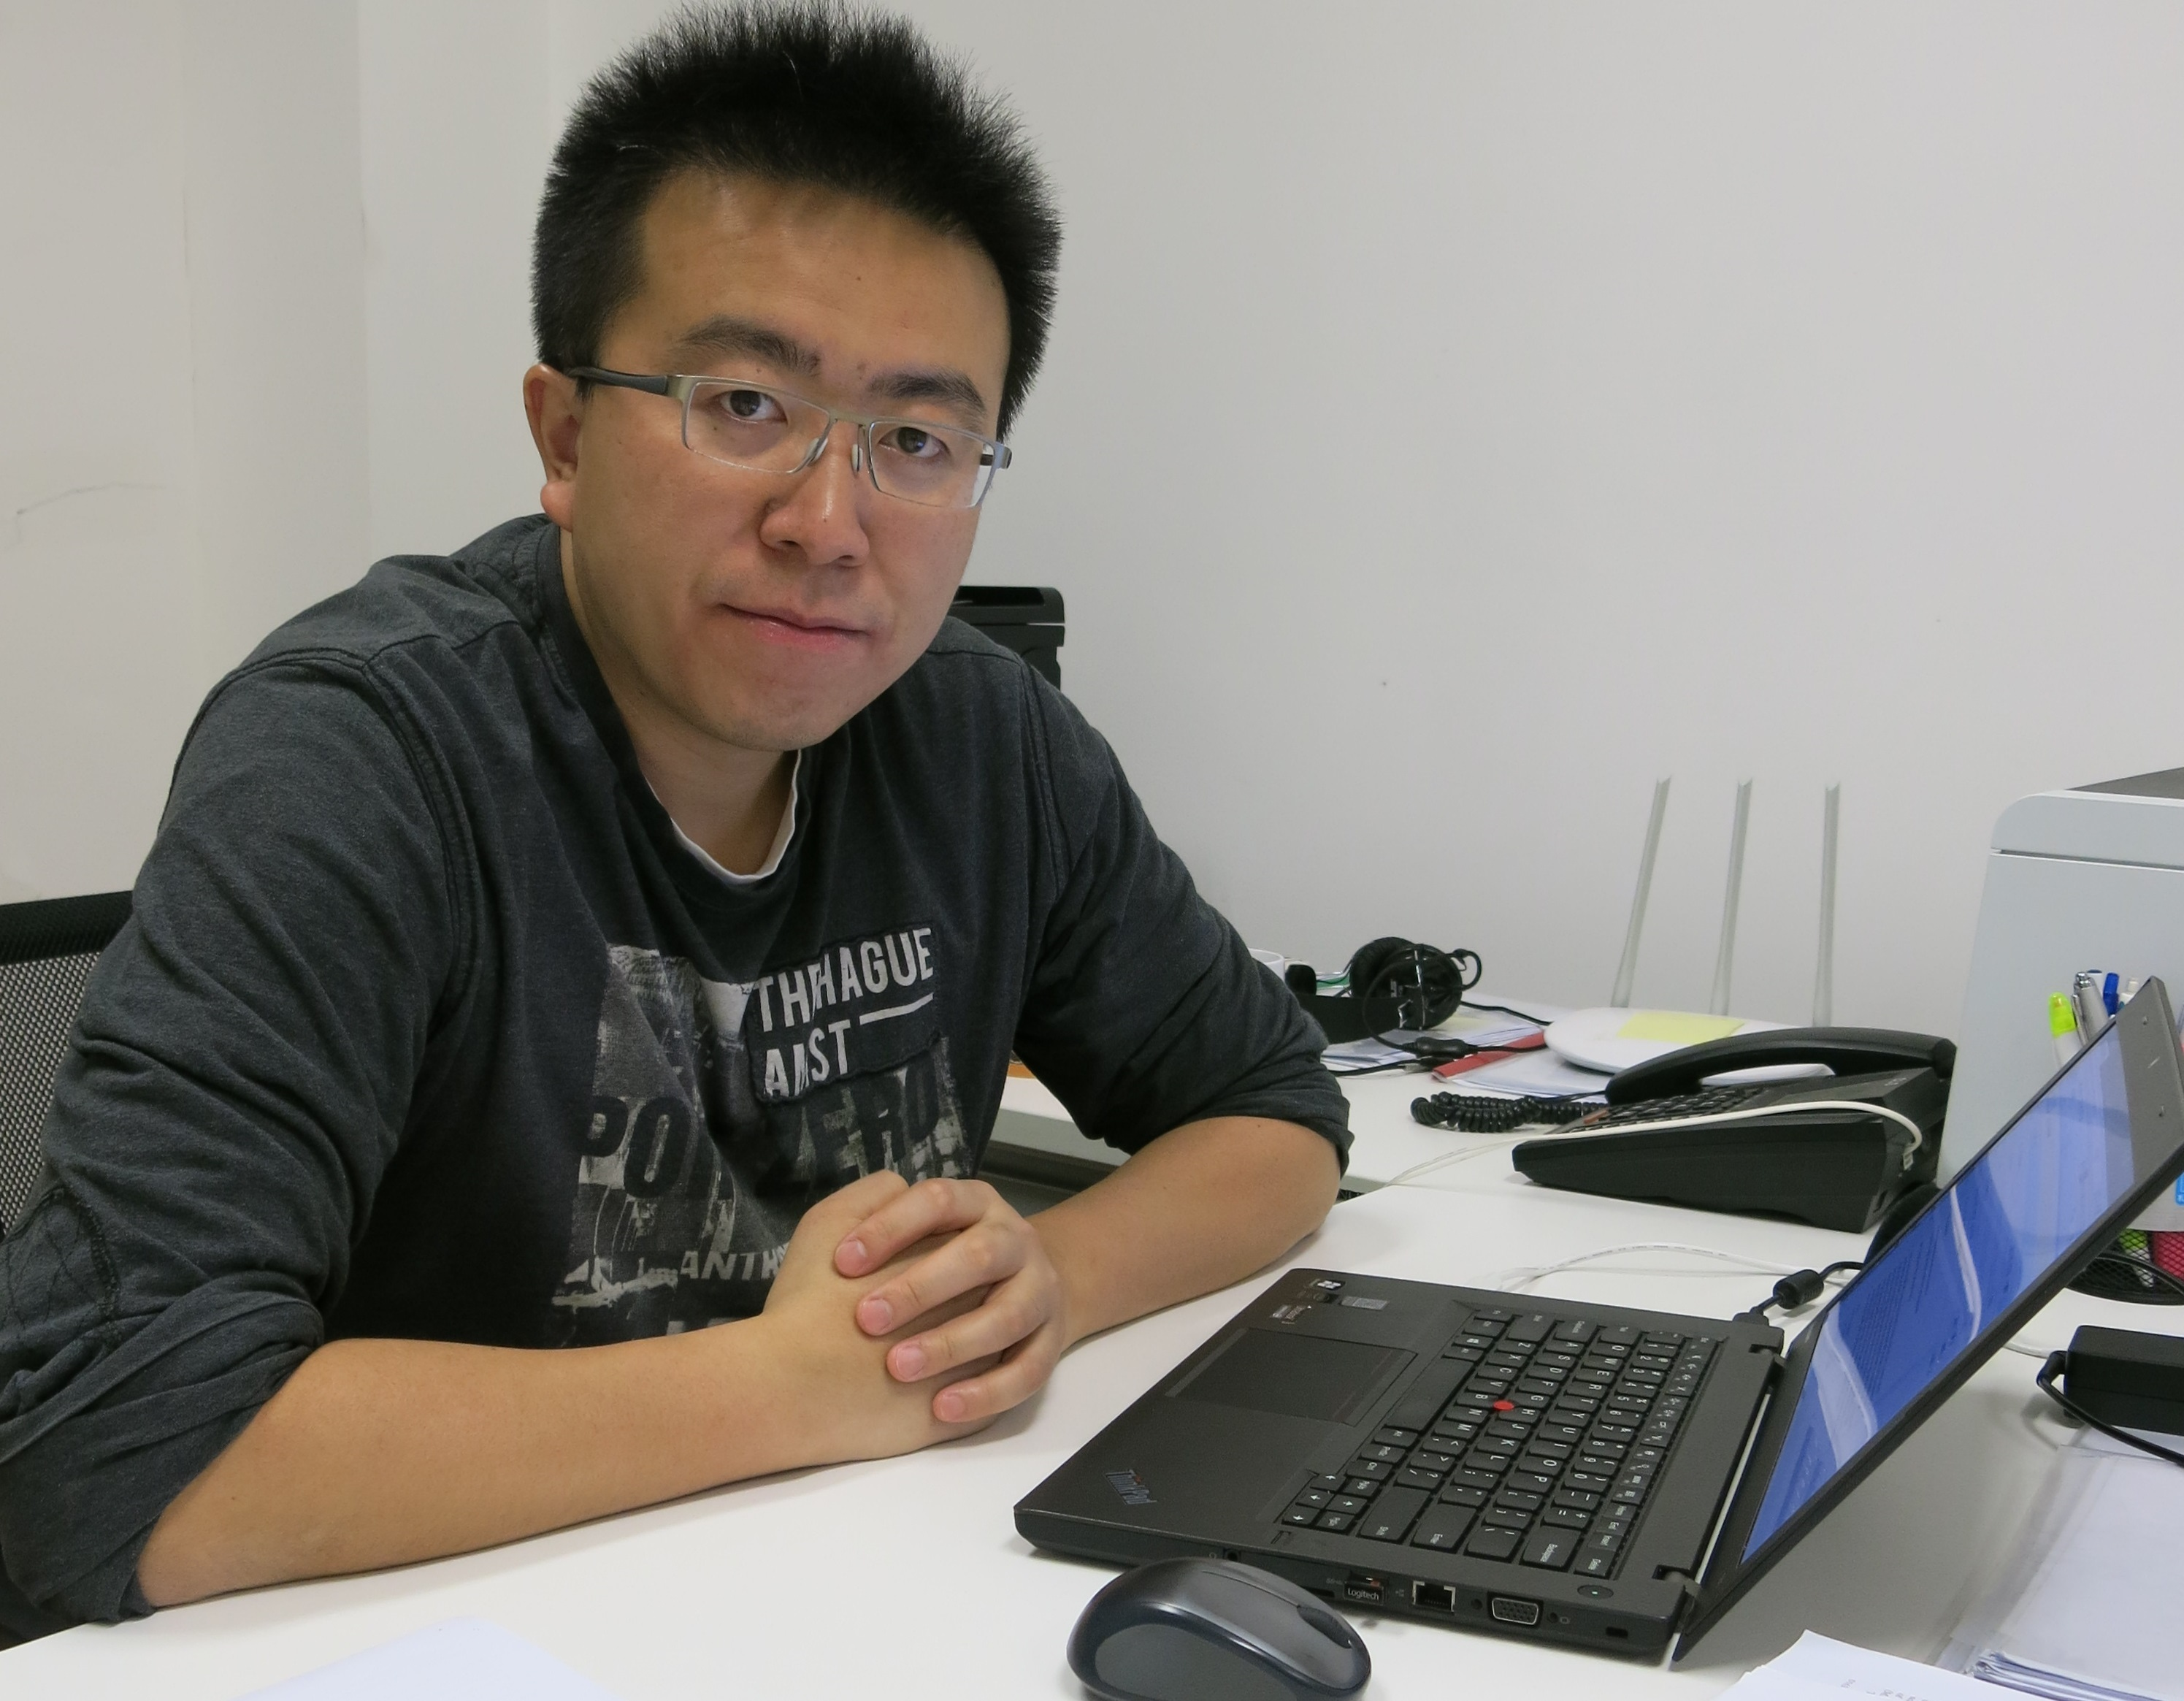
\includegraphics[height=2.5cm]{../people/ziyangmeng}\\
  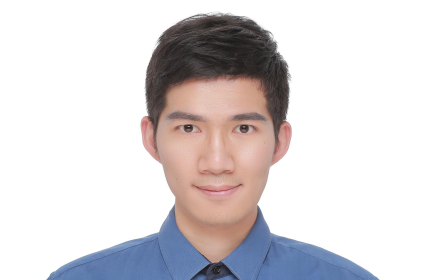
\includegraphics[height=2.5cm]{../people/xiaoyanxu}
  \includegraphics[height=2.5cm]{../people/kaisun}
\end{center}
\end{itemize}
\begin{center}
  \small arXiv:1801.00127
\end{center}
\end{frame}

\begin{frame}{Outline}
	%\begin{columns}
	%\column{.7\textwidth}
		\tableofcontents
  %\end{columns}
  % You might wish to add the option [pausesections]
\end{frame}

\section{Introduction: fermion QCPs and why they are hard.}

\begin{frame}
  \frametitle{Critical Points and Universal Behaviors}
  \begin{itemize}
  \item Universality class: critical points in different systems exhibit the same universal behavior.
  \item Example: 3D liquid-gas critical point and 2D transverse-field Ising model.
  \[H = -\sum_{\langle ij\rangle}\sigma_i^z\sigma_j^z+h_x\sum_i\sigma_i^x
  +h_z\sum_i\sigma_i^z.\]
\end{itemize}
  \begin{table}
    \centering
    \renewcommand{\arraystretch}{1.5}
    \rowcolors{2}{black!20}{}
    \begin{tabularx}{\columnwidth}{cxx}
      \rowcolor{mbg}&\textcolor{white}{Liquid-gas}&\textcolor{white}{TFIM}\\
      Phase diagram & 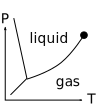
\includegraphics[width=2cm]{liquidgas} &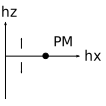
\includegraphics[width=2cm]{tfim}\\
      Order parameter & $\rho_l-\rho_g$ & $\sigma^z$\\
      Tuning field & $\alpha T+\beta P$ & $h_x$\\
      SB field & $\beta P-\alpha T$ & $h_z$
    \end{tabularx}
  \end{table}
\end{frame}

\begin{frame}
  \frametitle{Fermion QCPs}
  \begin{center}
    \includegraphics[width=\textwidth]{combine2}
  \end{center}
  \begin{itemize}
    \item Spin + fermion models.
    \item Spin ordering leads to spin density wave (SDW) instability on the Fermi Surface (FS).
    \item Different universality class: fermions on the FS are gapless excitations.
    \item Studying universal behaviors needs large lattice sizes, which is hard because the complexity of DQMC is $O(N^3)$.
  \end{itemize}
\end{frame}

\begin{frame}
  \frametitle{Determinant QMC}
  \begin{itemize}
    \item In general, DQMC simulations study the following fermion-boson models,
    \[H = H_f + H_{fb} + H_b\]
    \[H_f=-\sum_{ija}t_{ij}\left(c_{ia}^\dagger c_{ja}+\text{H.c.}\right)\]
    \[H_{fb}=\lambda\sum_ic_{ia}^\dagger M_{ab}c_{ib}\phi_i\]
    \item We sample bosonic field configurations $\{\phi\}$ with weights determined by integrating out the fermions:
    \[W[\phi] = W_b[\phi]\det(\mathbf I + \mathbf B(\beta,0;\phi))\]
    \item Hence the name ``determinant''.
    \item Complexity is \alert{$O(N^3)$}.
  \end{itemize}
\end{frame}

\begin{frame}
  \frametitle{Seeing universal behaviors is hard}
  \begin{itemize}
    \item Observing the universal behavior requires large system size: $L=30$ means $N=L^2=900$.
    \item \alert{$O(N^3)$} complexity is expensive.
  \end{itemize}
  \begin{center}
    
\includegraphics[height=4cm]{laptop_coffee}
    ~~~~~~~~~~~
    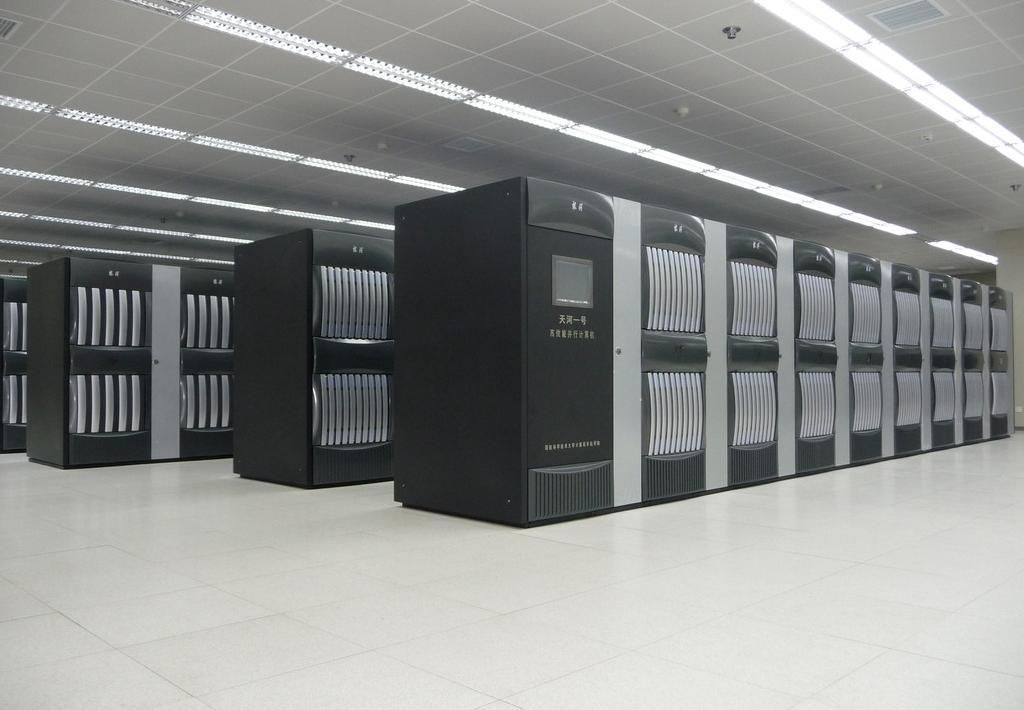
\includegraphics[height=4cm]{tianhe}
  \end{center}
\end{frame}

\section{EQMC: Elective Momentum Ultra-Size QMC}

\begin{frame}
  \frametitle{Elective momentum selection}
  \begin{center}
    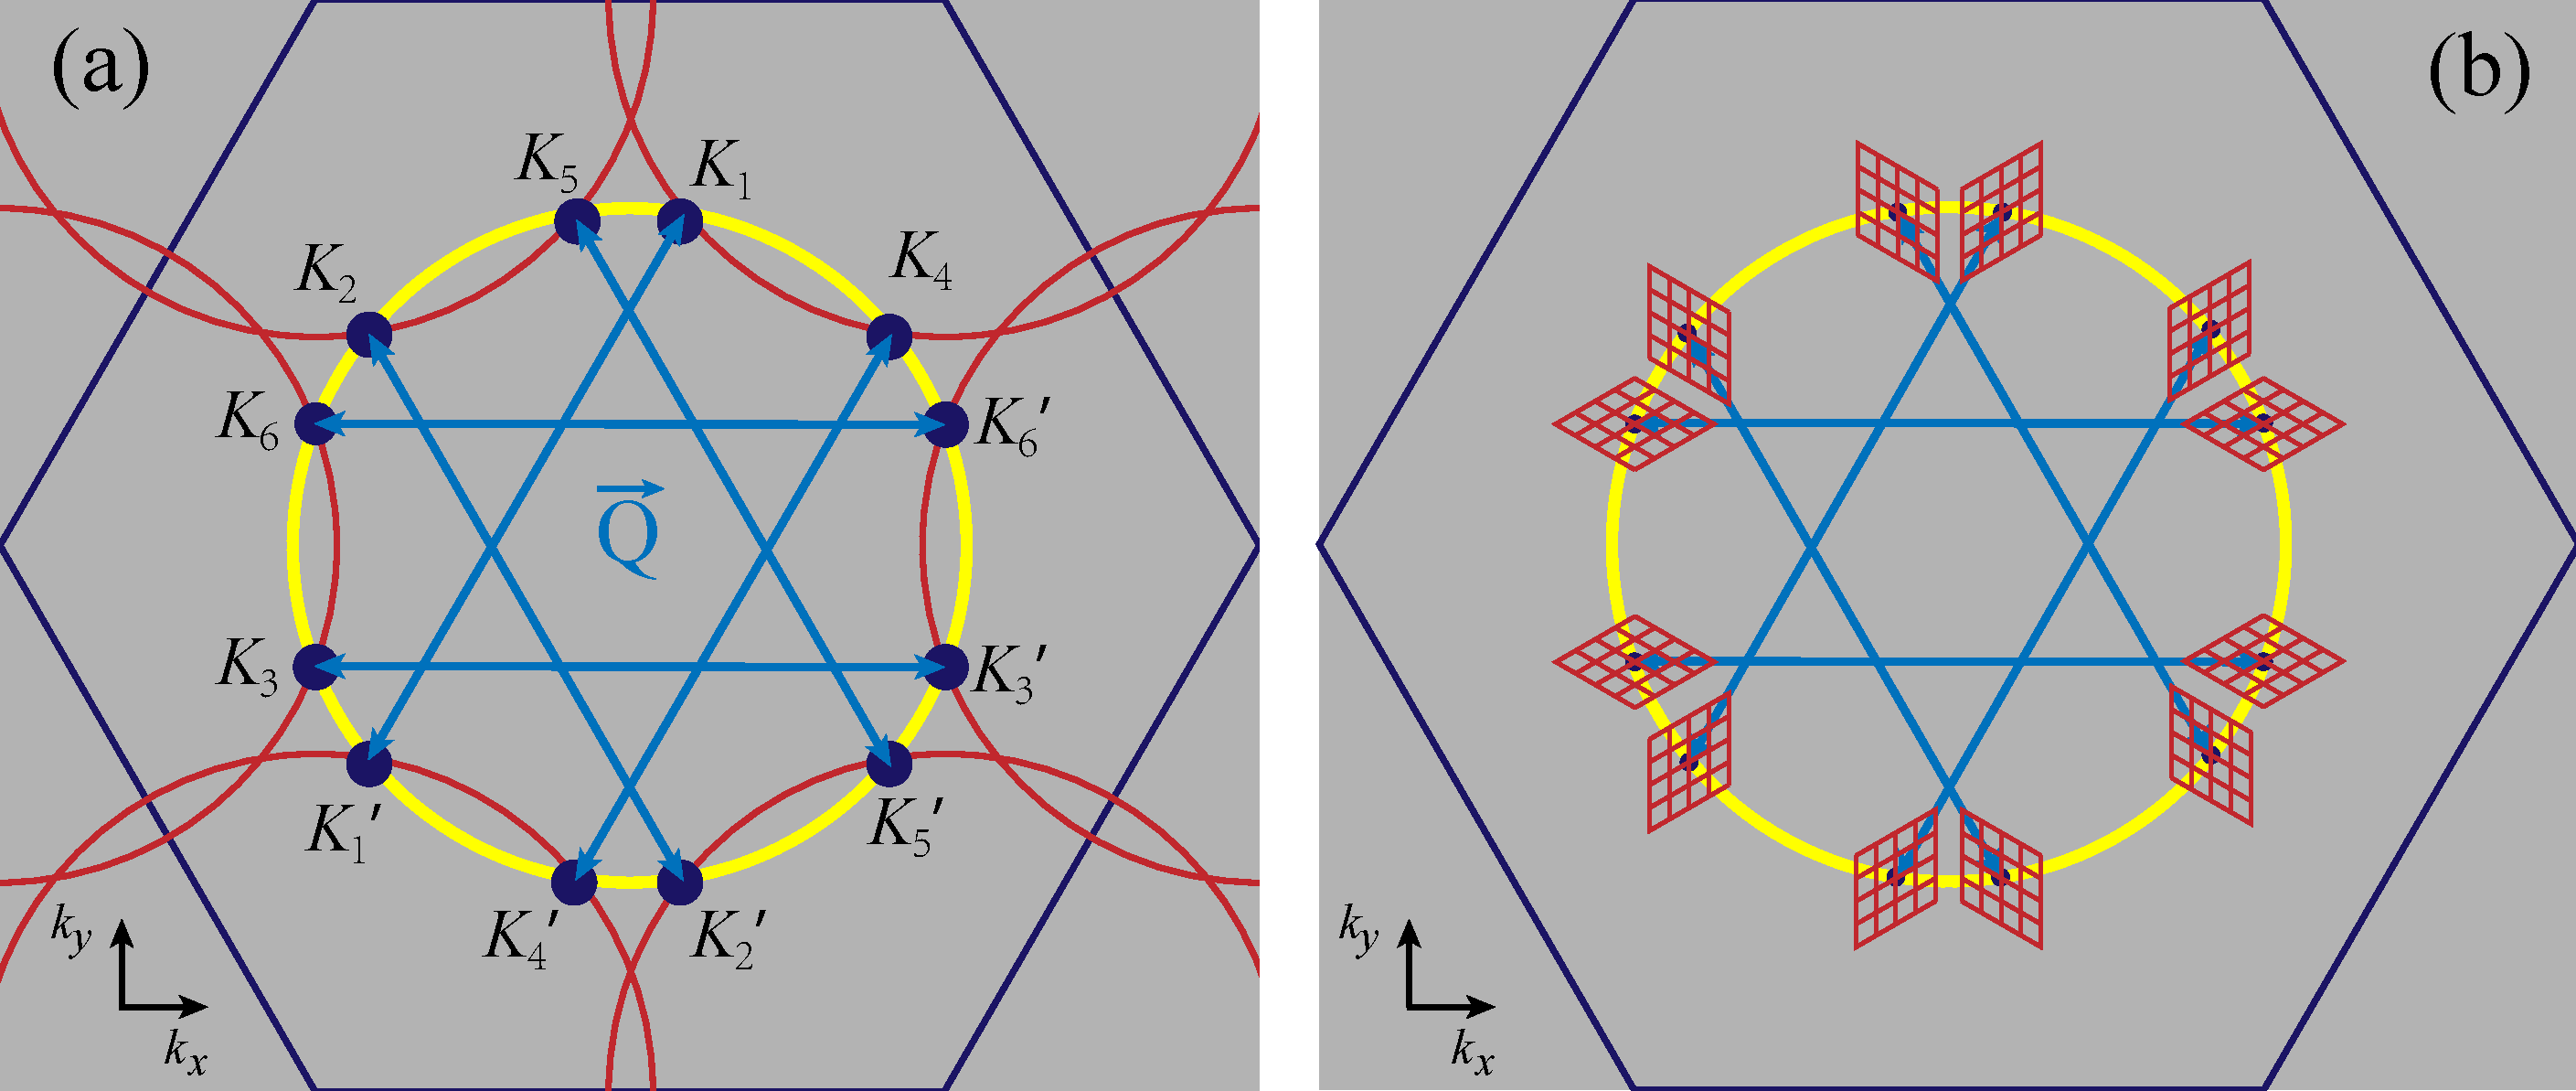
\includegraphics[width=.8\textwidth]{kmeshtri}
  \end{center}
\begin{itemize}
  \item Only $k$-modes near the ``hot spots'' contributes to the universal behaviors.
  \item In a lattice model, most modes are ``wasted'' as they only provide a UV completion.
  \item EQMC: only simulating $k$ modes inside patches.
  $O(N^3)\rightarrow O(N_f^3)$.
  \item Acceleration: $(N/N_f)^3$.
\end{itemize}
\end{frame}

\begin{frame}
  \frametitle{Working in the momentum space}
  \begin{table}
    \renewcommand{\arraystretch}{2.5}
    \rowcolors{2}{black!20}{}
  \begin{tabularx}{\columnwidth}{cxx}
    \rowcolor{mbg}
    & \textcolor{white}{Real space}
    & \textcolor{white}{Momentum space}\\
    $H_f = $ & $-\sum_{ija}t_{ij}(c_{ia}^\dagger c_{ja}+\text{H.c.})$
    & $\sum_k[\epsilon(k)-\mu]c_{ka}^\dagger c_{ka}$\\
    $H_{fb} = $
    & $\lambda\sum_ic_{ia}^\dagger M_{ab}c_{ib}\phi_i$
    & $\lambda\sum_{kk^\prime}c_{ka}^\dagger M_{ab}c_{k^\prime b}
    \alert<3>{\phi_{k-k^\prime}}$
  \end{tabularx}
  \end{table}
  \begin{itemize}
    \item We work in the momentum space.
    \item Only keep $k$ points within the patches.
  \end{itemize}
  Steps computing $W[\phi]$:
  \begin{enumerate}
    \item<2-4> Compute $W_b[\phi]$. Complexity $O(N)$
    \item<3-4> Fast Fourier Transform (FFT): $\phi_i\rightarrow\phi_k$. Complexity $O(N\log N)$.
    \item<4-5> Compute the fermion determinant. Complexity $O(N_f^3)$.
  \end{enumerate}
\end{frame}

\begin{frame}
  \frametitle{How to simulate: update algorithms?}
  \begin{block}{Local update for lattice models}
    \begin{itemize}
      \item In lattice models, bosons and fermions couple locally $\lambda\sum_ic_{ia}^\dagger M_{ab}c_{ib}\phi_i$.
      \item Flipping one spin $\phi_i$ changes only one column and one row of the fermion matrix
      \item The fast-update algorithm can the determinant with complexity $O(N)$. Scanning through the whole system: $N^2O(N)=O(N^3)$.
    \end{itemize}
  \end{block}
  \begin{itemize}
    \item Local update is not applicable: interaction is nonlocal in momentum space.
    \[\lambda\sum_{kk^\prime}c_{ka}^\dagger M_{ab}c_{k^\prime b}\phi_{k-k^\prime}\]
    \item We have to use global-update algorithms.
    \item We can use Self-Learning Monte Carlo (SLMC) algorithms.\\
    \emph{\small X-Y Xu, YQ, J Liu, L Fu and Z-Y Meng, PRB 96, 041119(R) (2017).}
    \item Complexity is $O(N_f^3)$.
  \end{itemize}
\end{frame}

\begin{frame}
  \frametitle{Update guided by an effective model}
  \begin{itemize}
    \item Detailed balance:
    \[\frac{p(\mathcal C\rightarrow\mathcal D)}{p(\mathcal D\rightarrow\mathcal C)}=\frac{W(\mathcal D)}{W(\mathcal C)}.\]
    %\item Detailed balance (and ergodicity) guarantees that if the MC converges, it converges to the desired distribution $W(\mathcal C)$.
    \item Metropolis-Hastings algorithm: propose -- accept/reject.
    \[p(\mathcal C\rightarrow\mathcal D) = q(\mathcal C\rightarrow\mathcal D)
    \alpha(\mathcal C\rightarrow\mathcal D).\]
    \[\alpha(\mathcal C\rightarrow\mathcal D) =
    \min\left\{1, \frac{W(\mathcal D)}{W(\mathcal C)}
    \frac{q(\mathcal D\rightarrow\mathcal C)}
    {q(\mathcal C\rightarrow\mathcal D)}\right\}.\]
    \item Guided by an effective model:
    \[\frac{q(\mathcal C\rightarrow\mathcal D)}
    {q(\mathcal D\rightarrow\mathcal C)}
    =\frac{W^\prime[\mathcal D]}{W^\prime[\mathcal C]}\]
    \[\alpha(\mathcal C\rightarrow \mathcal D)=\min\left\{1, \frac{W(\mathcal D)}{W(\mathcal C)}
    \frac{W^\prime(\mathcal C)}{W^\prime(\mathcal D)}\right\}\simeq1.\]
    \item Choice of $W^\prime$: $W_b$ or learned from SLMC.
  \end{itemize}
\end{frame}

\section{SLMC: A way to construct global updates}

\begin{frame}
  \frametitle{Design}
  \begin{center}
    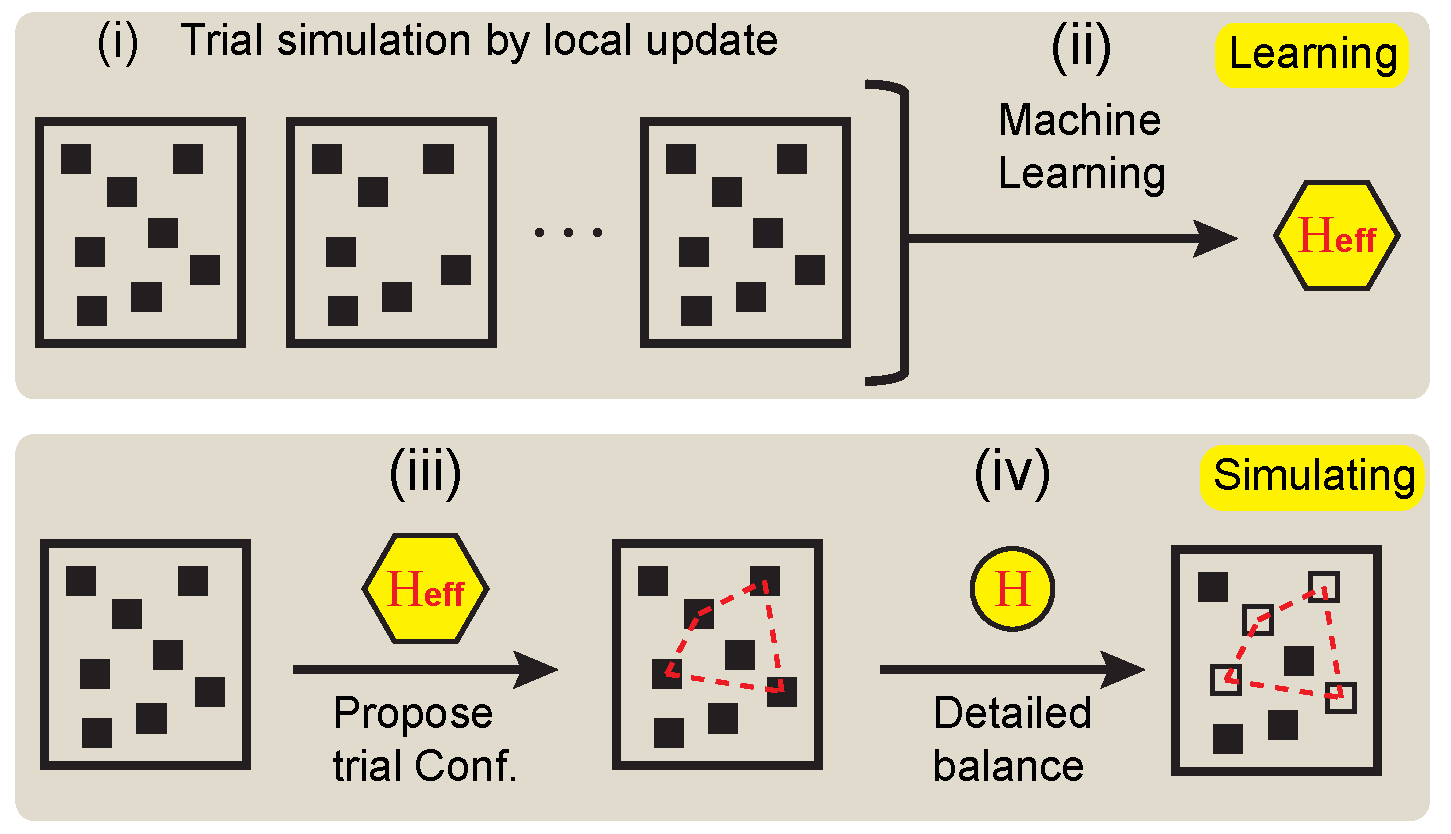
\includegraphics[width=\textwidth]{slmc-design}
  \end{center}
\end{frame}

\begin{frame}{Cumulative update}
  \begin{itemize}
    \item Idea: replace $W(\mathcal C)$ by $W^\prime(\mathcal C)$, which is much faster to evaluate.
    \item Local updates guided by $W^\prime(\mathcal C)$:
    \[\mathcal C\Rightarrow\mathcal D:
    \mathcal C\rightarrow\mathcal C_1\cdots\rightarrow\mathcal C_{i-1}\rightarrow\mathcal C_i\rightarrow\mathcal C_{i+1}\rightarrow\cdots\rightarrow\mathcal C_M\rightarrow\mathcal D.\]
    \item Detailed balance:
    \[\frac{p(\mathcal C_i\rightarrow\mathcal C_{i+1})}{p(\mathcal C_{i+1}\rightarrow\mathcal C_i)}=\frac{W^\prime(\mathcal C_{i+1})}{W^\prime(\mathcal C_i)}\]
    \item Selection rate:
    \[\frac{q(\mathcal C\rightarrow D)}
    {q(\mathcal D\rightarrow\mathcal C)}
    =\frac{W^\prime(\mathcal D)}{W^\prime(\mathcal C)}.\]
  \end{itemize}
\end{frame}

\begin{frame}{Cumulative update}
  \begin{itemize}
    \item Approximated weight:
    \[W^\prime(\mathcal C)\simeq W(\mathcal C).\]
    \item Update scheme:
    \[\frac{q(\mathcal C\rightarrow D)}
    {q(\mathcal D\rightarrow\mathcal C)}
    =\frac{W^\prime(\mathcal D)}{W^\prime(\mathcal C)}
    \simeq\frac{W(\mathcal D)}{W(\mathcal C)}.\]
    \item Acceptance ratio:
    \[\alpha(\mathcal C\rightarrow \mathcal D)=\min\left\{1, \frac{W(\mathcal D)}{W(\mathcal C)}
    \frac{W^\prime(\mathcal C)}{W^\prime(\mathcal D)}\right\}\simeq1.\]
    \item Choose good $W^\prime$ and $M\geq\tau_L$: $\tau_{CU}\sim1$.
    \item Computational cost: $\beta N^3\tau\rightarrow \beta N^3$.
    \item Again, $W^\prime(\mathcal C)\neq W(\mathcal C)$ does not introduce approximation.
  \end{itemize}
\end{frame}

\begin{frame}{Constructing effective weights}
\begin{enumerate}
  \item Physical intuition: bosonic effective model of $W_{\text{eff}}[\sigma]$
  + Linear Regression.\\
  \emph{Works best for gapped fermions.}
  \[H=-\sum_{ij}t_{ij}c_{i\alpha}^\dagger c_{j\alpha}
  +\sum_i\sigma_ic_{i\alpha}^\dagger\sigma^z_{\alpha\beta} c_{i\beta}
  +H[\sigma]\]
  \[W_{\text{eff}}[\sigma]=\sum_{ij}J_{ij}\sigma_i\sigma_j.\]
  \item Machine Learning models: todo in the future.
  \begin{itemize}
    \item Restricted Boltzmann Machine.
    \item Neural Networks.
  \end{itemize}
\end{enumerate}
\end{frame}

\begin{frame}{References}
\begin{itemize}
%\item Works led by Liang Fu, Zi-Yang Meng, and Lei Wang.
\item MIT: Jun-Wei Liu (HKUST), Hui-Tao Shen, Yuri Nagai, Liang Fu.
\item IOP: Xiao-Yan Xu (HKUST), Zi-Yang Meng.
\item References:
\begin{enumerate}
  \item J Liu, YQ, Z-Y Meng and L Fu, PRB 95, 041101(R) (2017).
  \item J Liu, H Shen, YQ, Z-Y Meng and L Fu, PRB 95, 241104(R) (2017).
  \item \alert{X-Y Xu, YQ, J Liu, L Fu and Z-Y Meng, PRB 96, 041119(R) (2017).}
  \item Y Nagai, H Shen, YQ and L Fu, PRB 96, 161102(R) (2017).
\end{enumerate}
\end{itemize}
\end{frame}


\section{Results: Benchmarking against regular DQMC}

\begin{frame}
  \frametitle{Hertz-Millis Theory}
  Scaling behavior:
\[\chi(T,h,\mathbf{q},\omega_n)=
\frac{1}{(\alert<3>{c_{t}T}+\alert<2>{c_{t}' T^{2}})
+c_{h}|h-h_c|^{\gamma}+c_q|\mathbf{q}|^2
+ (\alert<3>{c_{\omega}\omega}+\alert<2>{c'_{\omega}\omega^{2}})}\]
\begin{itemize}
  \item<2-> Bosonic QCP: $T^2\sim\omega^2\sim \bm q^2$.
  \item<3-> Fermionic QCP: $T\sim\omega\sim \bm q^2$.
  \item<4-> Crossover behavior:
  \begin{align*}
    \chi^{-1}(T\rightarrow0,h_c,0,\omega)-\chi^{-1}(T\rightarrow0,h_c,0,0))
    &\sim c_\omega\omega + c_\omega^\prime\omega^2.\\
    \chi^{-1}(T\rightarrow0,h_c,\bm q,0)-\chi^{-1}(T\rightarrow0,h_c,0,0))
    &\sim c_q|\bm q|^2.
  \end{align*}
\end{itemize}
\end{frame}

\begin{frame}
  \frametitle{Benchmarking against a previous work}
  \begin{center}
    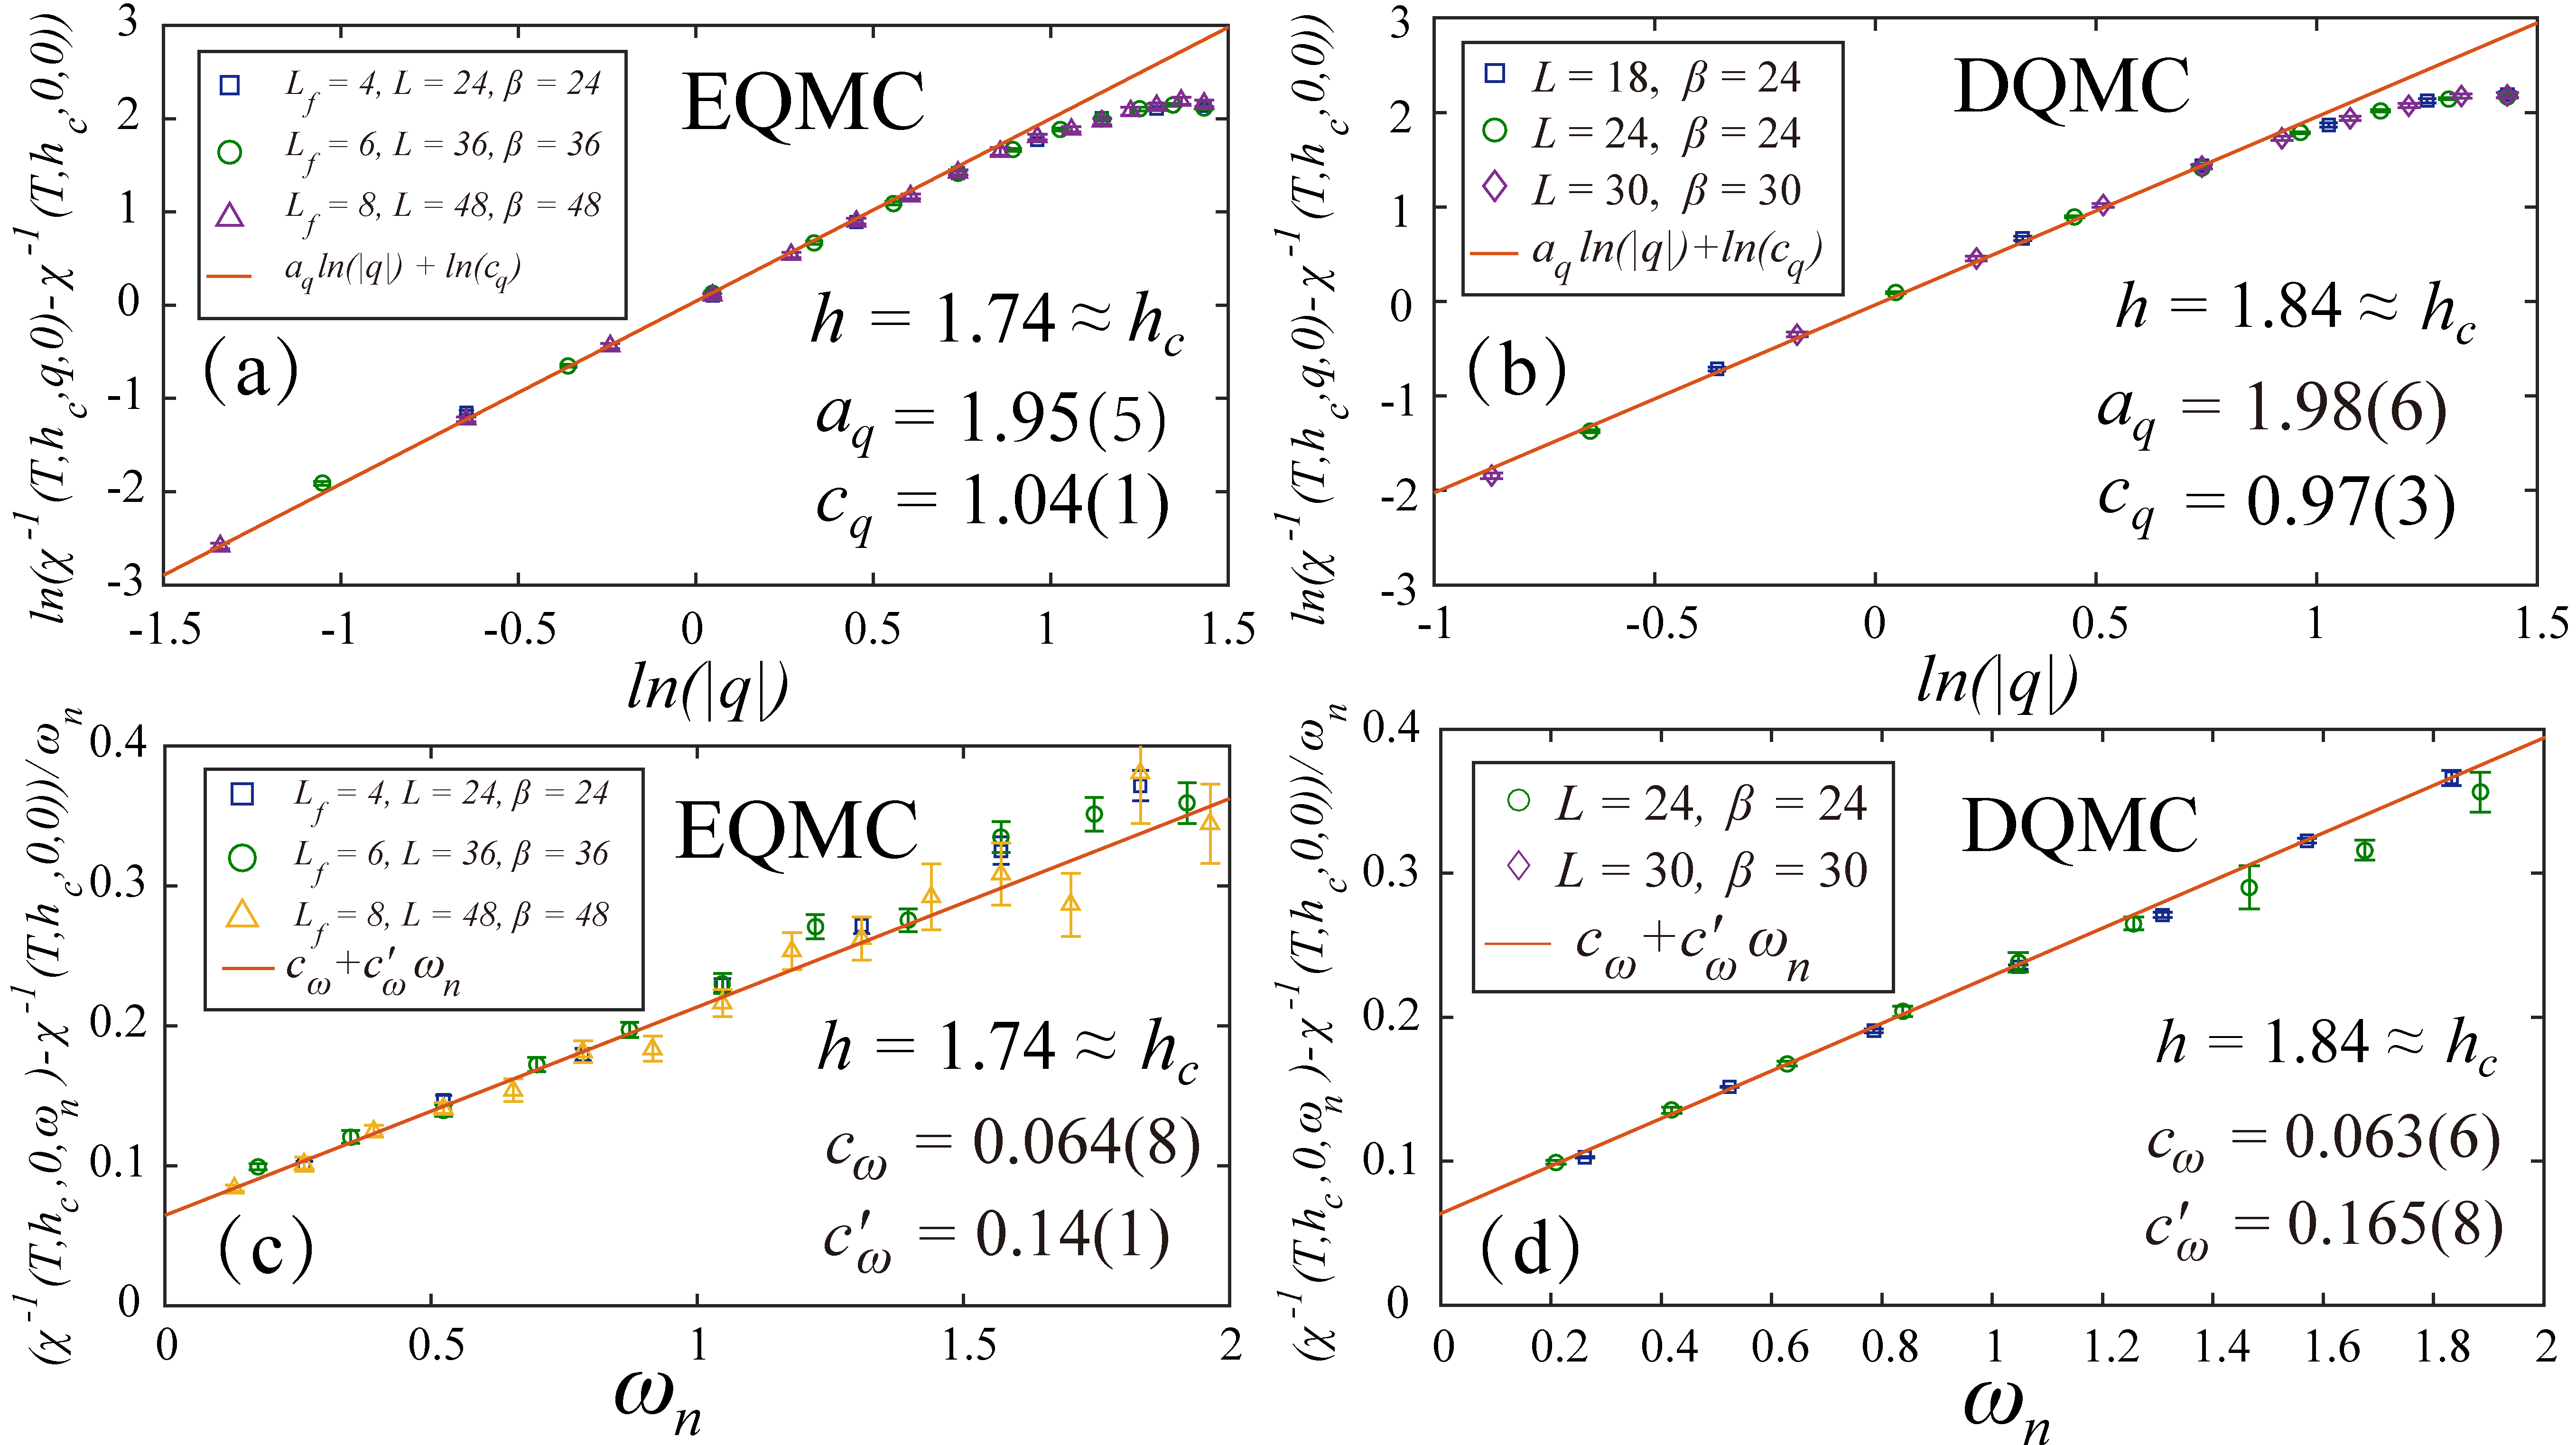
\includegraphics[width=\textwidth]{chiwqanalysis.pdf}
  \end{center}
\begin{itemize}
  \item Same scaling behaviors, quantitatively different results.
  \item Acceleration: $N/N_f=6^2=36$, $\frac1{12}(N/N_f)^3 \sim 10^4$.
\end{itemize}
\end{frame}

\section{Conclusion}

\begin{frame}
  \frametitle{Conclusion}
  \begin{itemize}
    \item EMUS-QMC Method: Hand-pick momentum-space patches included in DQMC simulations.
    \item Obtain the same IR universal physics with $(N/N_f)^3$ acceleration.
    \item EQMC is simulating a \alert{different} model, which exhibits the same universal behaviors.
    \item Useful for cases where UV completion is difficult.
  \end{itemize}
  \begin{center}
    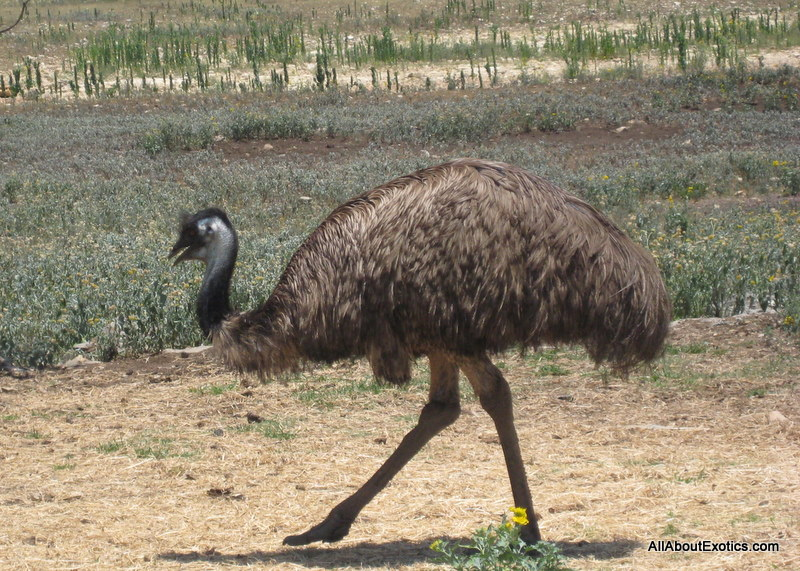
\includegraphics[height=3cm]{emu}
    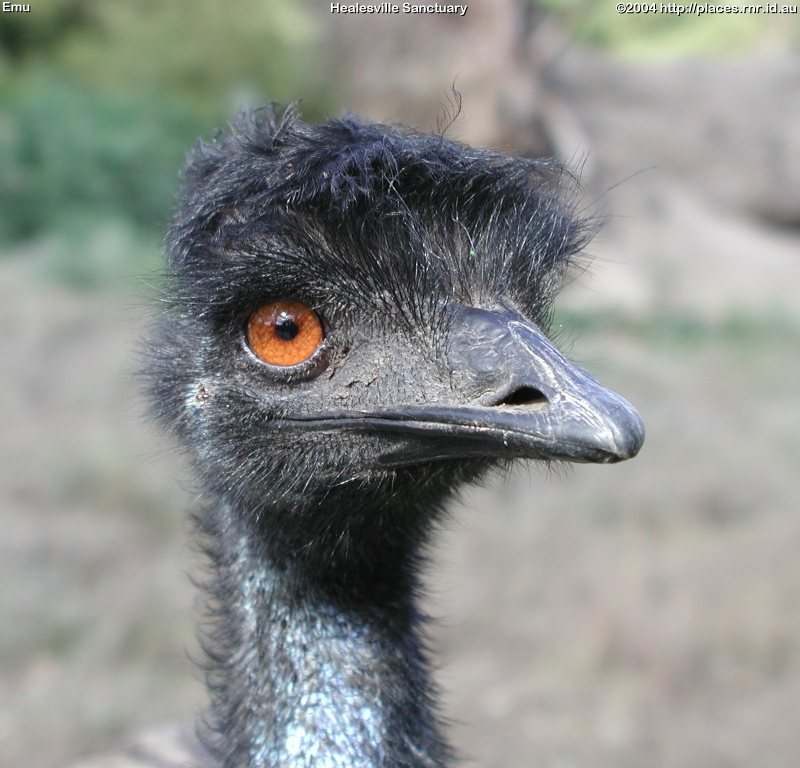
\includegraphics[height=3cm]{emu2}
  \end{center}
\end{frame}

\end{document}
